%%%%%%%%%%%%%%%%%%%%%%% file template.tex %%%%%%%%%%%%%%%%%%%%%%%%%
%
% This is a general template file for the LaTeX package SVJour3
% for Springer journals.          Springer Heidelberg 2010/09/16
%
% Copy it to a new file with a new name and use it as the basis
% for your article. Delete % signs as needed.
%
% This template includes a few options for different layouts and
% content for various journals. Please consult a previous issue of
% your journal as needed.
%
%%%%%%%%%%%%%%%%%%%%%%%%%%%%%%%%%%%%%%%%%%%%%%%%%%%%%%%%%%%%%%%%%%%
%
%
\RequirePackage{fix-cm}
%
%\documentclass{svjour3}                     % onecolumn (standard format)
\documentclass[smallcondensed]{svjour3}     % onecolumn (ditto)
%\documentclass[smallextended]{svjour3}       % onecolumn (second format)
%\documentclass[twocolumn]{svjour3}          % twocolumn
%
\smartqed  % flush right qed marks, e.g. at end of proof
%
\usepackage{graphicx}
%
%\usepackage{mathptmx}      % use Times fonts if available on your TeX system
%
% insert here the call for the packages your document requires
%\usepackage{latexsym}
% etc.
%
% please place your own definitions here and don't use \def but
% \newcommand{}{}
%
% Insert the name of "your journal" with
\journalname{Journal of Global Optimization}
%
\begin{document}

\title{Parallel global optimization on GPU 
	\thanks{The research is supported by the grant of the Ministry of education and science of the Russian Federation (the agreement of August 27, 2013 No 02.B.49.21.0003)}
}
%\subtitle{Do you have a subtitle?\\ If so, write it here}
%\titlerunning{Short form of title}        % if too long for running head

\author{Konstantin Barkalov         \and
        Victor Gergel 
}

%\authorrunning{Short form of author list} % if too long for running head

\institute{K. Barkalov  \at
              Computing Mathematics and Cybernetics Faculty, Lobachevsky State University of Nizhni Novgorod, Nizhni Novgorod, Russia \\
              Tel.: +7-831-4623356\\
              Fax: +7-831-4623085\\
              \email{barkalov@vmk.unn.ru} 
           \and
           V. Gergel \at
							\email{gergel@unn.ru} 
}

\date{Received: date / Accepted: date}
% The correct dates will be entered by the editor


\maketitle

\begin{abstract}
This work considers a parallel algorithm of solution of multidimensional multiextremal optimization problems. This algorithm uses Peano-type space filling curves for dimension reduction. Conditions of non-redundant parallelization of the algorithm is considered. The issue of implementation of the algorithm on modern computing systems with use of a graphics processing unit (GPU) is investigated. Speedup of the algorithm using GPU as compared with the same algorithm implemented on CPU only is demonstrated experimentally. Computing experiments are carried out on a series of several hundred of multidimensional multiextremal problems.
\keywords{Global optimization \and Parallel computing \and Graphics processing unit \and Peano-type space filling curves \and Characteristical algorithms}
% \PACS{PACS code1 \and PACS code2 \and more}
% \subclass{MSC code1 \and MSC code2 \and more}
\end{abstract}

\section{Introduction} \label{intro}

This present paper considers parallel algorithms for the solution of problems of multiextremal optimization. The objective function in such problems is characterized by existence of several local optima (usually their number is not known and can be large). In multiextremal problems the possibility of a reliable estimation of the global optimum is essentially based on the availability of a priori information about the function, allowing us to link possible values of an optimizable function with known values in search points. Very often, such information about the solvable problem is presented as the assumption that the objective function $\varphi$ satisfies a Lipschitz condition with a priori unknown constant $L$. The objective function can be represented by the algorithm of calculation of its values in the search domain, i.e. it can be a ``black-box'' function. Similar problems are widespread in applications (problems of optimal design of objects and technological processes in various fields of technology, problems of model fitting according to observed data in scientific research, optimization of control processes, etc., see the review \cite{RefPinter}).

Multiextremal optimization problems offer little in terms of analytical solution and numerical solution is computationally challenging as computational costs often grow exponentially in dimension. Employing modern parallel computational systems broadens the area of applicability of global optimization methods and, at the same time, poses a problem of efficient parallelization of the global search process. Therefore development of efficient parallel methods for numerical solution of multiextremal optimization problems and their software implementation for modern computational systems is the main direction of research in this area.

One of the promising directions of development in the field of parallel global optimization (as in many areas connected with software implementation of complex algorithms) is the use of graphics processing units (GPUs). During the last decade, productivity of GPUs has been rapidly growing to satisfy the continuously growing demand of graphic application developers. Furthermore, some principles of development of graphics hardware have changed over the past few years, and it became more programmable. Today a GPU is a high-performance flexibly programmable and massively parallel processor that can provide solution to many computationally complex problems \cite{RefHwu}.

However, in the domain of global optimization the potential of GPUs is not completely unlocked. GPUs are generally used for parallelization of algorithms, which one way or another are based on the concept of random search (see works \cite{RefFerreiro,RefZhu,RefGarcia,RefMussi}); a review of this direction of GPU optimization algorithms is given in \cite{RefLangdon}. Owing to their stochastic nature, algorithms of this type generally do not guarantee convergence to a globally optimal solution, and that sets them apart from deterministic methods.

For many deterministic algorithms of Lipschitzian global optimization with guaranteed convergence parallel variants are proposed \cite{RefGergel2005,RefEvtushenko,RefHe,RefPaulavicius}. However, these versions of algorithms are parallelized on CPU using MPI and/or OpenMP technologies; there are no implementations on GPU. The present article contains the results of an investigation into the GPU implementation of the global search parallel algorithm developed according to the information-statistical approach presented in the monograph \cite{RefStrongin2000}.

The main part of the paper has the following structure. Section \ref{sec:2} contains a description of the basic algorithm of global search. Section \ref{sec:3} contains a scheme of its parallelization, and section \ref{sec:4} includes theoretical statements that characterize the speedup and non-redundancy of the parallel algorithm. In section \ref{sec:5}, ways of possible implementation of the parallel algorithm on GPU are discussed. Section \ref{sec:6} contains the results of numerical experiments; a comparison of the sequential algorithm and parallel CPU and GPU versions for solving a series of test multidimensional multiextremal problems is also made. Section \ref{sec:7} concludes the paper.

\section{Multidimensional global search algorithm} \label{sec:2}

Let us consider the problem of search for a global minimum of an $N$-dimensional function $\varphi(y)$ within a hyper interval $D$
\begin{eqnarray}\label{eq:1}
& \varphi(y^\ast)=\min{\left\{\varphi(y):y\in D\right\}},\\
& D=\left\{y\in R^N: a_i\leq y_i \leq b_i, 1\leq i \leq N\right\}. \nonumber
\end{eqnarray}

Let us assume that the function $\varphi$ satisfies a Lipschitz condition with a priori unknown constant $L$
\[
\left|\varphi(y_1)-\varphi(y_2)\right|\leq L\left\|y_1-y_2\right\|,\; y_1,y_2 \in D,\; 0<L<\infty.
\]

There is a number of ways to adapt effective one-dimensional algorithms for solving multidimensional problems; see, for example, the diagonal partitions method in \cite{RefSergeyev2006} or the simplicial partitions method in \cite{RefZilinskas}. In this paper, we will use the approach based on the idea of dimension reduction by means of a Peano curve $y(x)$, which continuously and unambiguously maps the unit interval [0,1] onto the $n$-dimensional cube
\[
\left\{y\in R^N: -2^{-1}\leq y_i \leq 2^{-1}, 1 \leq i \leq N\right\}=\left\{y(x):0\leq x \leq 1 \right\}.
\]
Problems of numerical construction of Peano-type space filling curves and the corresponding theory are considered in detail in \cite{RefStrongin2000}, \cite{RefSergeyev2013}. Here we will note that a numerically constructed curve (\textit{evolvent}) is an approximation to a theoretical Peano curve with an accuracy $2^{-m}$ , where $m$ is an evolvent construction parameter. It means that using evolvent we can distinguish points in a multidimensional space, the coordinates of which differ by not less than $2^{-m}$; closer points are considered as coincident. Thereby an evolvent constructed with a fixed m allows obtaining a solution of a problem with an accuracy of not more than $2^{-m}$ by coordinate.

By using mapping of this kind it is possible to reduce the multidimensional problem~(\ref{eq:1}) to a one-dimensional problem
\[
\varphi(y^\ast)=\varphi(y(x^\ast))=\min{\left\{\varphi(y(x)): x\in[0,1]\right\}}.
\]
An important property is preservation of boundedness of function relative differences  (see \cite{RefStrongin2000}): if the function $\varphi(y)$ in the domain $D$ satisfies the Lipschitz condition, then the function $\varphi(y(x))$ on the interval $[0,1]$ will satisfy a uniform H{\"o}lder condition
\[
\left|\varphi(y(x_1))-\varphi(y(x_2))\right|\leq H\left|x_1-x_2\right|^{1/N},
\]
where the H{\"o}lder constant $H$ is linked to the Lipschitz constant $L$ by the relation
\[
H=4Ld\sqrt{N},\;\; d=\max{\left\{b_i-a_i:1\leq i \leq N\right\}}.
\]

Therefore, it is possible, without limitation of generality, to consider minimization of one-dimensional function
\[
f(x)=\varphi(y(x)), \;\; x\in[0,1],
\]
satisfying the H{\"o}lder condition.

The considered algorithm for solving this problem (here, according to \cite{RefStrongin2000}) assumes constructing a sequence of points $x^k$, where the values of minimized function $z^k = f(x^k)$ are calculated. Let us call the process of calculating the function value (including the construction of an image $y^k=y(x^k)$) the ``trial'', and the pair $(x^k, z^k)$ --  the ``trial result''. Set of pairs $\left\{(x^k, z^k)\right\}, 1\leq k\leq n,$ make up the search data collected using the method after carrying out $n$ steps. The rules that determine the work of the global search algorithm are as follows.

At the first iteration of the method the trial is carried out in arbitrary internal point $x^1$ of interval $[0,1]$. The point of trial at the next iteration $(k+1)$ is determined according to these rules.

Step 1. Renumber points of the set
\[
X_k=\{x^1,\dots,x^k\}\cup\left\{0\right\}\cup\left\{1\right\},
\]
which includes boundary points of interval $[0,1]$ and points of the previous trials, with subscripts in increasing order of coordinate values, i.e.
\[
0=x_0<x_1<\dots <x_k<x_{k+1}=1.
\]

Step 2. Supposing that  $z_i=f(x_i), \; 1\leq i \leq k$, calculate values 
\begin{equation}\label{eq:11}
\mu = \max_{2\leq i \leq k}\frac{\left|z_i-z_{i-1}\right|}{\Delta_i},
\end{equation}
\[
M = \left\{
   \begin{array}{lr}
     r\mu, & \mu > 0,\\
     1, & \mu = 0,
   \end{array}
\right.
 \]
where $r>1$ is a preset parameter of the method, and $\Delta_i=\left(x_i-x_{i-1}\right)^{1/N}$.

Step 3. Calculate \textit{characteristic} for every interval $(x_{i-1}, x_i), \; 1\leq i \leq k+1,$   according to the following formulas
\[
R(1)=2\Delta_1-4\frac{z_1}{M},
\]
\begin{equation}\label{eq:14}
R(i)=\Delta_i+\frac{(z_i-z_{i-1})^2}{M^2\Delta_i}-2\frac{z_i+z_{i-1}}{M},1<i<k+1,
\end{equation}
\[
R(k+1)=2\Delta_{k+1}-4\frac{z_k}{M}.
\]

Step 4. Find interval $(x_{t-1},x_t)$ with maximum characteristic
\[
R(t)=\max{\left\{R(i): 1 \leq i \leq k+1\right\}}.
\]

Step 5. Carry out a trial in point $x^{k+1}\in(x_{t-1},x_t)$, calculated using the following formulas
\[
x^{k+1} = \frac{x_t+x_{t-1}}{2}, \textrm{ if } t=1 \textrm{ or } t=k+1,
\]
\[
x^{k+1} = \frac{x_t+x_{t-1}}{2} - \mathrm{sign}(z_t-z_{t-1})\frac{1}{2r}\left[\frac{\left|z_t-z_{t-1}\right|}{\mu}\right]^N, \textrm{ if } 1<t<k+1.
\]

The algorithm stops working if the condition $\Delta_t<\epsilon$ is satisfied; here $\epsilon>0$ the accuracy is preset. For estimation of the global solution values
\[
f_k^\ast=\min_{1\leq i \leq k}f(x^i), \ x_k^\ast=\arg \min_{1\leq i \leq k}f(x^i).
\]
are selected.

Remark 1. The normalized characteristics $R(i)$ from (\ref{eq:14}) can be viewed as probabilities of locating of a global minimize within the interval $[x_{i-1},x_i], 1\leq i \leq k+1$. This statement is proved in \cite{RefStrongin2000}. Thus, at each iteration a new trial point is selected inside the interval, which has the greatest probability of finding a global minimum. 

Remark 2. The proof of convergence of this algorithm is provided in \cite{RefStrongin2000}. The modifications considering existence of inequality constraints in the problem and information about objective function derivative are given in \cite{RefBarkalov,RefGergel1996,RefGergel1997}.

Let us illustrate the work of this \textit{global search algorithm} (GSA) using a dimension reduction for minimization of a two-dimensional multiextremal function
\begin{eqnarray} \nonumber \label{eq:19}
\varphi(y)= -&\left\{\left(\sum^{7}_{i=1}\sum^{7}_{j=1}A_{ij}g_{ij}(y)+B_{ij}h_{ij}(y)\right)^2+\right. \\
&\left.\left(\sum^{7}_{i=1}\sum^{7}_{j=1}C_{ij}g_{ij}(y)+D_{ij}h_{ij}(y)\right)^2\right\}^{1/2},\\ \nonumber
\end{eqnarray}
where
\begin{eqnarray} \nonumber
& y=(y_1,y_2)\in R^2, 0 \leq y_s \leq 1, s=1,2, \\ \nonumber
& g_{ij}(y)=\sin(i\pi y_1)\sin(j\pi y_2),  \\ \nonumber
& h_{ij}(y)=\cos(i\pi y_1)\cos(j\pi y_2), \nonumber 
\end{eqnarray}
and coefficients $A_{ij}, B_{ij}, C_{ij}, D_{ij}$  are taken uniformly in interval $[-1,1]$. The experiment used method parameters $r=3$, $\epsilon=10^{-3}$, and evolvent construction parameter $m=12$. Fig.~\ref{fig:1} shows contour lines of one of functions generated according to (\ref{eq:19}) and points of 1103 trials carried out using the method before the required accuracy was obtained.
\begin{figure}
	\center
  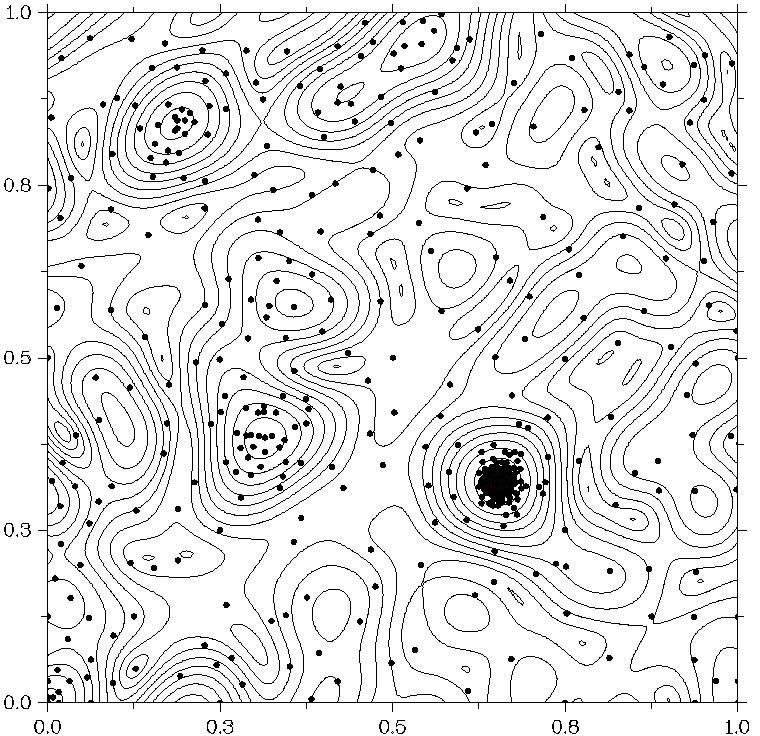
\includegraphics[width=0.75\textwidth]{fig1.jpg} 
  \caption{Minimization of two-dimensional function}
  \label{fig:1}       % Give a unique label
\end{figure}

\section{Synchronous parallel algorithm} \label{sec:3}

Let us now consider $p>1$ computing elements (cores in CPU or GPU). In this case, search process parallelization can be organized in several ways.

First, it is possible to parallelize calculation of the target function describing the optimized object. This method can provide speedup, but is specific for each solved problem.

Secondly, it is possible to parallelize implementation of algorithm computing rules providing selection of the point of the next trial. In this case the way of parallelization will depend on the class of algorithms and, besides, these rules are often rather simple and it is inexpedient to parallelize them (overhead costs of the organization of parallelism will reduce possible speedup to zero).

Thirdly, it is possible to change the scheme of algorithm for the purpose of carrying out several trials in parallel. This approach is the most promising since it is characterized by efficiency (the part of computing process, in which the bulk of calculations is carried out, is parallelized) and generality (it is applicable for a wide class of characteristical algorithms of multiextremal optimization \cite{RefGrishagin1997}).

Let us describe a change of rules of global search algorithm for the purpose of simultaneous (synchronous) carrying out in one iteration of method $p$ of trials. Let us make $k(n)$ the total number of trials, carried out after $n$ of parallel iterations.

Suppose $n\geq 1$  iterations of the method are carried out, in which trials were performed in $k=k(n)$ points $x^i,1\leq i \leq k$. Then points $x^{k+1},\dots,x^{k+p}$  of search trials of the next $n+1$ iteration are determined according to the rules.

Steps 1--3 of the parallel algorithm fully repeat steps 1--3 of the global search algorithm.

Step 4. Arrange characteristics  $R(i), 1 \leq i \leq k+1$, in decreasing order 
\begin{equation}\label{eq:21}
R(t_1)\geq R(t_2)\geq \dots \geq R(t_{k}) \geq R(t_{k+1})
\end{equation}
and select $p$ maximum characteristics with interval numbers $t_j, 1\leq j \leq p$.

Step 5. Carry out new trials in points $x^{k+j}\in(x_{t_j-1},x_{t_j}), 1\leq j\leq p$, calculated using formulas
\[
x^{k+j} = \frac{x_{t_j}+x_{t_j-1}}{2}, \textrm{ if } t_j=1 \textrm{ or } t_j=k+1,
\]
\[
x^{k+j} = \frac{x_{t_j}+x_{t_j-1}}{2} - \mathrm{sign}(z_{t_j}-z_{t_j-1})\frac{1}{2r}\left[\frac{\left|z_{t_j}-z_{t_j-1}\right|}{\mu}\right]^N, \textrm{ if } 1<t_j<k+1.
\]

The algorithm stops working if the condition $\Delta_{t_j}<\epsilon$ is satisfied at least for one number $t_j, 1 \leq j \leq p$ ; $\epsilon>0$ is the preset accuracy.  For estimation of the global solution values
\[
f_k^\ast=\min_{1\leq i \leq k}f(x^i), \ x_k^\ast=\arg \min_{1\leq i \leq k}f(x^i).
\]
are selected.

The modifications of the parallel algorithm considering information about the minimized function derivative are given in \cite{RefGergel1999}.

This method of organizing parallel computing has the following justification \cite{RefStrongin2000,RefGrishagin1997}. The characteristics of intervals (\ref{eq:14}) used in the algorithm of global search can be considered as probability measures of location of the global minimum point in these intervals. Inequalities (\ref{eq:21}) arrange intervals according to their characteristics, and trials are carried out in parallel in the first $p$ intervals with the largest probabilities.

Let us use a parallel algorithm of global search for solution of a problem from section \ref{sec:2} with numbers of parallel trials $p=2$ and $p=4$. With $p=2$ the number of iterations was $569$, and the number of trials was $1138$. With $p=4$ the number of iterations was reduced to $270$, and $1080$ trials were carried out. Contour lines of the function are shown in Fig.~\ref{fig:2} with points of the trials carried out by the method when using $p=4$. Points of redundant trials carried out using a parallel algorithm are marked in the figure by "+". In more detail the concept of redundancy is discussed in the following section.
\begin{figure}
	\center
  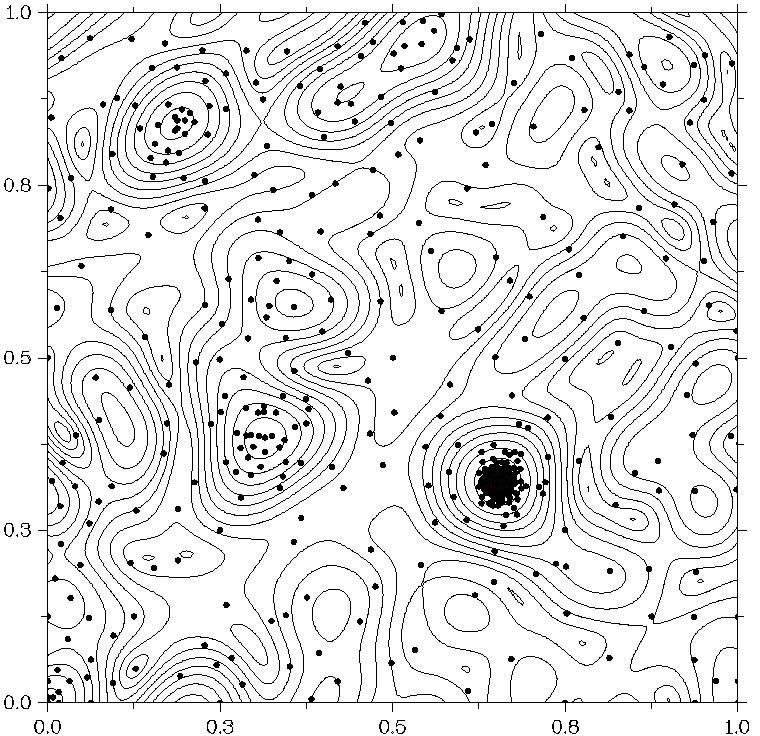
\includegraphics[width=0.75\textwidth]{fig2.jpg} 
  \caption{Minimization of a two-dimensional function by a parallel algorithm}
  \label{fig:2}
\end{figure}

\section{Speedup and non-redundancy of a parallel algorithm} \label{sec:4}

Let us describe theoretical properties of a parallel algorithm, which characterize its speedup. One of the main indicators of efficiency of parallel algorithms (in any domain, not only in global optimization) is speedup in time
\[
S(p)=T(1)/T(p),
\]
where $T(1)$ is the time spent for solution of a problem by a sequential algorithm, and $T(p)$ is the time of solution of the same problem by a parallel algorithm in a system with $p$ computing elements. The characteristic of efficiency of parallel algorithms (in relation to algorithms of optimization) is also speedup in number of iterations
\begin{equation}\label{eq:26}
s(p)=n(1)p/n(p),
\end{equation}
where $n(1)$ is the number of the trials carried out using the sequential method, and $n(p)$ is the number of the trials carried out using the parallel method with p processors. This characteristic is especially important since for solution of applied problems the time of carrying out of a trial exceeds the time of processing of its results.

It is obvious that number of trials $n(p)$ for sequential and parallel algorithms described in sections \ref{sec:2} and \ref{sec:3} will differ. Actually, the sequential algorithm of global search when selecting point $x^{k+1}$ of the next $k+1$ trial possesses complete information received at the previous $k$ iterations. The parallel algorithm of global search selects not one, but $p$ points $x^{k+j}, 1\leq j \leq p$,  at iteration $k+1$ based on the same information. It means that selection of point $x^{k+j}$ is carried out in absence of information on the trial results in points $x^{k+i}, 1\leq i<j$. Only the first point $x^{k+1}$ will coincide with the point selected by the sequential algorithm. Points of the other trials generally can not coincide with the points generated by the sequential algorithm. Carrying out of such trials can reduce efficiency of use of parallel processors. Therefore, let us consider such trials as ``redundant'', and the value 
\[
\lambda(p) = \left\{
   \begin{array}{lr}
     (n(p)-n(1))/n(p), & n(p) > n(1),\\
     0, & n(p)\leq n(1),
   \end{array}
\right.
\]
as ``method redundancy''.

Let us set the series of trials $\left\{x^k\right\}$ and $\left\{y^m\right\}$ generated correspondingly by sequential and parallel algorithms for solution of the same problem with $\epsilon = 0$ in the condition of stopping. The following theorem from \cite{RefStrongin2000} determines the number of computing elements $p$, which can be involved for non-redundant parallelization.

\textbf{Theorem}. Suppose $x^\ast$ is the point of global minimum, $x'$ is the point of the local minimum of function $f(x)$, and the following conditions are fulfilled:
\begin{enumerate}
	\item
	Inequality 
	\begin{equation}\label{eq:28}
	f(x')-f(x^\ast)\leq \delta, \delta>0,
	\end{equation}
	holds.
	\item
	The initial $q(l)$ trials of the sequential and parallel methods coincide, i.e.
	\[
	\left\{x^1,\dots,x^{q(l)}\right\}=\left\{y^1,\dots,y^{q(l)}\right\},
	\]
	where 
	\[
	\left\{x^1,\dots,x^{q(l)}\right\}\subset\left\{x^k\right\}, \ \left\{y^1,\dots,y^{q(l)}\right\}\subset\left\{y^m\right\}.
	\]
	\item
	There exists a point $y^n\in \left\{y^m\right\}, n<q(l),$ such that $x'\leq y^n \leq x^\ast$ or \mbox{$x^\ast \leq y^n \leq x'$}.
	\item
	For value $M$ from (\ref{eq:11}) the following inequality
	\[
	M>2^{2-1/N}H
	\]
	holds, where $H$ is H{\"o}lder constant of the minimized function.
\end{enumerate}

Then a parallel algorithm of global search using two processors will be non-redundant (i.e. $s(2)=2$, $\lambda(2)=0$) while the following condition is satisfied 
\begin{equation}\label{eq:32}
\left(x_{t_j}-x_{t_j-1}\right)^{1/N} > \frac{4\delta}{M-2^{2-1/N}H}, 1\leq j\leq p,	
\end{equation}
where $t_j$ are determined according to (\ref{eq:21}).

\textbf{Corollary}. Let the objective function $f(x)$ have $Q$ local minimum points $\left\{x'_1,\dots,x'_Q\right\}$, for which condition (\ref{eq:28}) is fulfilled, and let there exist trial points $y^{n_i}, 1\leq i \leq Q,$ such as
\[
y^{n_i}\in \left\{y^1,\dots,y^{q(l)}\right\},
\]
\[
\alpha_i \leq y^{n_i} \leq \alpha_{i+1}, \; \alpha_i, \alpha_{i+1} \in \left\{x^\ast, x'_1,\dots,x'_Q\right\}, \; 1\leq i \leq Q.
\]

Then, if the theorem conditions are satisfied, the parallel algorithm of global search with $Q+1$ processors will be non-redundant (i.e. $s(Q+1)= Q+1$, \mbox{$\lambda(Q+1)=0$}), while condition (\ref{eq:32}) is satisfied.

The theorem corollary plays a special role for solution of multidimensional problems reduced to one-dimensional problems by means of Peano-like evolvent $y(x)$. Evolvent $y(x)$, which is approximation to Peano curve, has the effect of ``splitting'' of a point of the global minimum $y^\ast\in D$ to several preimages in interval $[0,1]$. If function $\varphi(y)$ has the only global minimum in $D$, the ``reduced'' function $f(x)$ can have up to $2^N$ local extremum points close (by value) to a global extremum point (see \cite{RefStrongin2000}). In case of applying a parallel global search algorithm for minimization of a similar function it is possible receive non-redundancy when using up to $2^N+1$ computing elements.

The parallel algorithm of global search showed a good speedup in implementation on CPU in systems with a small number of processors. In \cite{RefGrishagin1997,RefStrongin2003} a speedup of algorithm close to linear was experimentally verified when carrying out 2-4 parallel trials. The results of work of the parallel GSA for minimization of 100 two-dimensional multiextremal functions described by formula (\ref{eq:19}) are shown in table \ref{tab:1}. All experiments used method parameters $r=2.9$, and $\epsilon=10^{-3}$, and the global minimum was found with the demanded accuracy in all $100$ problems. The table shows the number of used processors $p$, the average number of trials $n(p)$ rounded to integers and average speedup in iterations $s(p)$ from (\ref{eq:26}). 

\begin{table}
	\caption{Results of minimization of $100$ two-dimensional functions}
	\label{tab:1}
	\center
	\begin{tabular}{lll}
		\hline\noalign{\smallskip}
		 $p$ & $n(p)$ & $s(p)$ \\
		\noalign{\smallskip} \hline \noalign{\smallskip}
			1 &	1575 &	\dots \\
			2 &	1596 &	1.97 \\
			3 &	1562 &	3.02 \\
			4 &	1599 &	3.94 \\
		\noalign{\smallskip}\hline
	\end{tabular}
\end{table}

\section{Implementation on GPU} \label{sec:5}

What advantages does GPU have in case of implementation of global optimization algorithms? First, CPU has only a small (up to $16$ in the advanced models) number of cores working independently at a high clock frequency. Each CPU core is a powerful computer. GPU, on the contrary, works at low clock frequencies and uses hundreds of simpler computing elements. Second, a considerable share of a CPU crystal is occupied by a high-speed cache memory, while practically the whole of GPU consists of arithmetic and logic units. Therefore, GPUs are especially effective in problems, in which the number of arithmetic operations is great in comparison with memory operations.

With respect to methods of global optimization, the operation which can be implemented effectively on GPU is simultaneous parallel computing of many values of the objective function. Naturally, for this purpose the function value calculation procedure has to be implemented on GPU. Transfers of information from CPU to GPU will be minimal: it is necessary only to transfer to GPU coordinates of trial points and to receive values of the function in these points. The functions that determine the processing of trial results according to algorithm and require work with a large volume of collected search information can be effectively implemented on CPU.

A general scheme of organization of calculations using GPU is shown in Fig.~\ref{fig:3}. According to this scheme steps 1 -- 4 of a parallel global search algorithm are carried out on a CPU. The coordinates of $p$ points of trials calculated at step 4 of the algorithm are collected in an intermediate buffer, and then are transferred to the graphics processing unit. Calculation of function values in these points is carried out on GPU, and then the results of trials (again via the intermediate buffer) are transferred to CPU.

\begin{figure}
	\center
  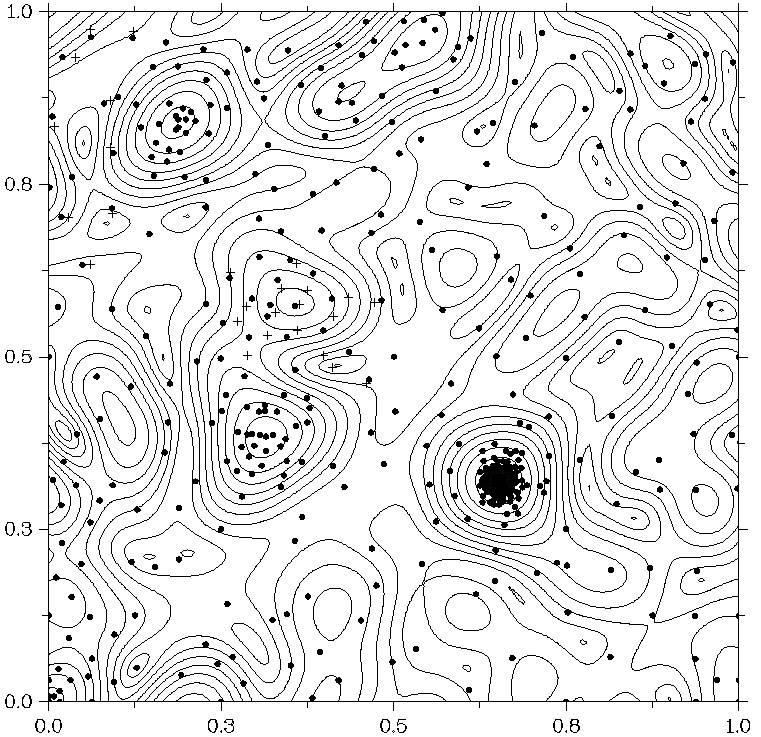
\includegraphics[width=0.75\textwidth]{fig3.jpg} 
  \caption{Scheme of information exchanges in a GPU algorithm}
  \label{fig:3}
\end{figure}


The use of several hundred of parallel computing elements (as in modern GPU) might not give a speedup of the search process by hundreds of times. In this case, conditions of the theorem of non-redundant parallelization can be violated: the number of local extremums will be less than the number of computing cores. Then (according to the theorem and its corollary) a parallel GSA will generate redundant trial points. Nevertheless, despite certain redundancy, the general operating time of a GPU algorithm will be less than the operating time of a CPU algorithm. This has been verified by computing experiments, the results of which are given in section \ref{sec:6}.

\section{Results of numerical experiments} \label{sec:6}

Computing experiments were carried out on one of the nodes of a high-performance cluster of the State University of Nizhny Novgorod. The cluster node includes 2 Intel Sandy Bridge E5-2660 2.2 GHz CPUs, 64 Gb RAM, and NVIDIA Tesla M2090 GPU. The CPU has 8 cores (i.e. 16 physical cores and 16 virtual cores in hyper-threading mode are available in the node). The graphics processing unit includes 16 multiprocessors (512 cores). For implementation of the GPU algorithm CUDA Toolkit 6.0 was used.

Keep in mind that widely known test problems from the domain of multidimensional global optimization are characterized by small time of objective function values calculation. Usually, such a calculation is nothing else than a summation of several (according to problem dimension) values of elementary functions. For example, the well known Rastrigin’s test function, the global minimum of which is located in $y^\ast = (0,\dots,0)$ with $\varphi(y^\ast)=0$, is set by the expression
\begin{equation}\label{eq:33}
\varphi(y)=10N+\sum^{N}_{i=1}\left[y^2_i-10\cos(2\pi y_i)\right], \; -2.2\leq y_i \leq 1.8, \; 1\leq i \leq N.
\end{equation}

Therefore, for the purpose of imitation of the computational complexity inherent to applied problems of optimization \cite{RefBarkalov2013}, calculation of the objective function in all performed experiments was complicated by additional calculations without changing the type of function and arrangement of its minimums (series summation from 20 thousand elements).

It is noteworthy that an important parameter for starting any GPU program (unlike a parallel program on CPU) is not only the number of threads $p$, but also the size of the \textit{thread block}. Separate threads on GPU are grouped in blocks of threads of identical size, thus each thread block is executed on a separate multiprocessor. Threads in a thread block can interact effectively using information in shared memory and synchronization. For the purpose of assessing the importance of the size of a thread block during the period of execution of a GPU algorithm let us perform a preliminary series of experiments with the test function (\ref{eq:33}) with $N=5$. Let us vary the number $p$ of the used GPU threads and the size $pB$ of a thread block. All the other parameters of the method do not change ($r=2.3$, $\epsilon = 10^{-3}$, the evolvent construction parameter $m=10$). Table \ref{tab:2} shows the GPU algorithm operating time depending on $p$ and $pB$.
\begin{table}
	\caption{GPU algorithm operating time depending on thread block size}
	\label{tab:2}
	\center
	\begin{tabular}{llllll}
		\hline\noalign{\smallskip}
%		 $p$ & $pB=16$ & $pB=32$ & $pB=64$ & $pB=128$ & $pB=256$  \\
		$p$ & \multicolumn{5}{l}{ \hfil $pB$ \hfil } \\
		\noalign{\smallskip} \cline{2-6} \noalign{\smallskip}
		 & 16 & 32 & 64 & 128 & 256  \\
		\noalign{\smallskip} \hline \noalign{\smallskip}
		100 &	39.43 &	41.5 &	39.71 &	39.85 &	39.61 \\
		300 &	24.84 &	24.52 &	24.54 &	24.66 &	25.08 \\
		500 &	9.25 &	9.45 &	9.24 &	9.4 &	9.3\\
		700 &	11.8 &	13.43 &	11.78 &	11.91 &	12.03\\
		900 &	10.9 &	10.91 &	10.85 &	10.86 &	10.96\\
		1000 &	10.92 &	10.8 &	10.76 &	10.9 &	10.74\\
		\noalign{\smallskip}\hline
	\end{tabular}
\end{table}

As is seen from this table, there is a speedup of the algorithm in the case of an increase in the number of trials at one iteration up to the number of cores on GPU, with subsequent saturation. Owing to a weak information dependence the size of the thread block $pB$ does not have determining influence, therefore let us use $pB=64$ in all subsequent experiments. When carrying out this set of experiments the load on GPU was 15 -- 85 \% (depending on the number of threads); the load was measured by GPUZ program.

After fixing the GPU parameters let us make the main computing experiments on a series of multidimensional multiextremal problems. In work \cite{RefGaviano} a GKLS generator allowing generation of multiextremal optimization problems with known properties (number of local minima, size of their domains of attraction, global minimum point, function value, etc.) is described.  

The results of numerical comparison of the three sequential algorithms -- DIRECT \cite{RefJones}, DIRECT\textit{l} \cite{RefGablonsky} and global search algorithm (GSA) from section \ref{sec:2} -- are provided below (results of work of the first two algorithms are given in paper \cite{RefGaviano}). Numerical comparison was carried out on function classes \textit{Simple} and \textit{Hard} of dimension 4 and 5 from \cite{RefGaviano} since the solution of problems of dimension 2 and 3 demands a small number of iterations and it is impractical to use GPU for solving these problems. Global minimum $y^\ast$ was considered to be found, if the algorithm generated trial point $y^k$ in $\delta$-vicinity of the global minimum, i.e. $\left\|y^k-y^\ast\right\|\leq\delta$. The size of the vicinity was selected (according to \cite{RefGaviano}) as $\delta = \left\|b-a\right\|\sqrt[N]{\Delta}$, $N$ -- problem dimension, $a$ and $b$ -- borders of search domain $D$, parameter $\Delta=10^{-6}$ at $N=4$ and $\Delta=10^{-7}$ at $N=5$. When using the GSA for the class \textit{Simple} parameter $r=4.5$ was selected, for the class \textit{Hard} $r=5.6$ was selected; Peano curve construction parameter was fixed as $m=10$. The maximum allowable number of iterations was $K_{max} = 10^6$.

The average number of iterations $k_{av}$ performed by the method for solving a series of problems from these classes is shown in table \ref{tab:3}. Symbol $>$ reflects a situation in which not all problems of the class were solved by the method. This means that the algorithm was stopped as the maximum allowable number of iterations $K_{max}$ was achieved. In this case, value $K_{max}=10^6$ was used for calculating the average value of the number of iterations $k_{av}$ that corresponds to the lower estimate of this average value. The number of unsolved problems is specified in brackets.

\begin{table}
	\caption{Average number of iterations $k_{av}$}
	\label{tab:3}
	\center
	\begin{tabular}{lllll}
		\hline\noalign{\smallskip}
  	 $N$ & Problem class & DIRECT & DIRECT\textit{l} & GSA \\
		\noalign{\smallskip} \hline \noalign{\smallskip}
			4 &	\textit{Simple}	& $>$47282(4) &	18983 &	11953 \\
	      & \textit{Hard} &	$>$95708(7) &	68754 &	25263 \\
			5	& \textit{Simple} &	$>$16057(1) &	16758 &	15920 \\
				& \textit{Hard} &	$>$217215(16) &	$>$269064(4) & $>$148342 (4) \\
		\noalign{\smallskip}\hline
	\end{tabular}
\end{table}

Table \ref{tab:3} shows that GSA outperforms DIRECT and DIRECT\textit{l} methods on all classes of problems by average number of iterations. And in class 5-\textit{Hard} each of the methods solved not all problems: DIRECT did not solve 16 problems, DIRECT\textit{l} and GSA -- 4 problems.

Let us estimate now the speedup when using the parallel global search algorithm implemented on CPU depending on the number $p$ of the used cores. Table \ref{tab:4} shows the average number of iterations performed by the method when solving a series of problems, and table \ref{tab:5} shows the average time requared to solve one problem. Tables \ref{tab:6} and \ref{tab:7} show speedup in time $S(p)$ and iterations $s(p)$ respectively; speedup of the parallel algorithm was measured in relation to the sequential one ($p=1$).

\begin{table}
	\caption{Average number of iterations on CPU}
	\label{tab:4}
	\center
	\begin{tabular}{llllll}
		\hline\noalign{\smallskip}
		$p$ & \multicolumn{2}{l}{ $N=4$ } & & \multicolumn{2}{l}{$N=5$} \\
		\noalign{\smallskip} \cline{2-3} \cline{5-6} \noalign{\smallskip}
		 & \textit{Simple} & \textit{Hard} & & \textit{Simple} & \textit{Hard}  \\
		\noalign{\smallskip} \hline \noalign{\smallskip}
		1 &	11953 &	25263 & &	15920 &	$>$148342(4) \\
		2 &	6014 &	16509 & & 17797 &	98667 \\
		4 &	2547 &	8970 & &	8246 &	45410 \\
		8 &	1413 &	4666 & &	3773 &	26732 \\
		16 &	756 &	1910 & &	1713 &	11322 \\
		32 &	323 &	1252 & &	781 &	11745 \\
		\noalign{\smallskip}\hline
	\end{tabular}
\end{table}

\begin{table}
	\caption{Average problem solution time on CPU}
	\label{tab:5}
	\center
	\begin{tabular}{llllll}
		\hline\noalign{\smallskip}
		$p$ & \multicolumn{2}{l}{ $N=4$ } & & \multicolumn{2}{l}{$N=5$} \\
		\noalign{\smallskip} \cline{2-3} \cline{5-6} \noalign{\smallskip}
		 & \textit{Simple} & \textit{Hard} & & \textit{Simple} & \textit{Hard}  \\
		\noalign{\smallskip} \hline \noalign{\smallskip}
		1 &	3.02 &	6.05 & &	4.84 &	$>$42.5 \\
		2 &	1.8 &	4.48 & &	5.84 &	33.77 \\
		4 &	1.0 &	2.94 & &	3.18 &	15.62 \\
		8 &	0.71 &	1.88 & &	1.82 &	14.16 \\
		16 &	0.57 &	1.36 & &	1.44 &	8.37 \\
		32 &	0.38 &	1.25 & &	0.95 &	11.67 \\
		\noalign{\smallskip}\hline
	\end{tabular}
\end{table}

\begin{table}
	\caption{Time speedup $S(p)$ on CPU}
	\label{tab:6}
	\center
	\begin{tabular}{llllll}
		\hline\noalign{\smallskip}
		$p$ & \multicolumn{2}{l}{ $N=4$ } & & \multicolumn{2}{l}{$N=5$} \\
		\noalign{\smallskip} \cline{2-3} \cline{5-6} \noalign{\smallskip}
		 & \textit{Simple} & \textit{Hard} & & \textit{Simple} & \textit{Hard}  \\
		\noalign{\smallskip} \hline \noalign{\smallskip}
		2 &	1.68 &	1.35 & &	0.83 &	$>$1.26 \\
		4 &	3.04 &	2.06 & &	1.52 &	2.72 \\
		8 &	4.27 &	3.22 & &	2.66 &	3.64 \\
		16 &	5.29 &	4.46 & &	3.36 &	5.08 \\
		32 &	8.04 &	4.85 & &	5.11 &	3.0 \\
		\noalign{\smallskip}\hline
	\end{tabular}
\end{table}


\begin{table}
	\caption{Iteration speedup $s(p)$ on CPU}
	\label{tab:7}
	\center
	\begin{tabular}{llllll}
		\hline\noalign{\smallskip}
		$p$ & \multicolumn{2}{l}{ $N=4$ } & & \multicolumn{2}{l}{$N=5$} \\
		\noalign{\smallskip} \cline{2-3} \cline{5-6} \noalign{\smallskip}
		 & \textit{Simple} & \textit{Hard} & & \textit{Simple} & \textit{Hard}  \\
		\noalign{\smallskip} \hline \noalign{\smallskip}
		2 &	1.99 & 1.53 & &	0.89 &	$>$1.50 \\
		4 &	4.69 &	2.82 & &	1.93 &	3.27 \\
		8 &	8.46 &	5.41 & &	4.22 &	5.55 \\
		16 &	15.82 &	13.23 & &	9.29 &	13.1 \\
		32 &	37.04 &	20.18 & &	20.39 &	12.63 \\
		\noalign{\smallskip}\hline
	\end{tabular}
\end{table}

\begin{table}
	\caption{Redundancy $\lambda(p)$ on CPU}
	\label{tab:8}
	\center
	\begin{tabular}{llllll}
		\hline\noalign{\smallskip}
		$p$ & \multicolumn{2}{l}{ $N=4$ } & & \multicolumn{2}{l}{$N=5$} \\
		\noalign{\smallskip} \cline{2-3} \cline{5-6} \noalign{\smallskip}
		 & \textit{Simple} & \textit{Hard} & & \textit{Simple} & \textit{Hard}  \\
		\noalign{\smallskip} \hline \noalign{\smallskip}
2 &	0.01 & 0.23 & &	0.55 &	$>$0.25 \\
4 &	0 &	0.3 & &	0.52	& 0.18 \\
8 &	0 &	0.32 & &	0.47  &	0.31 \\
16 &	0.01 &	0.17& &	0.42  &	0.18 \\
32 &	0 &	0.37 & &	0.36  &	0.61 \\
		\noalign{\smallskip}\hline
	\end{tabular}
\end{table}

The data show quintuple time speedup, when using 32 cores for all classes (except 5-\textit{Hard}). Delay in class 5-\textit{Hard} in transition from 16 to 32 cores is explained by an increase in average number of iterations and by the fact that out of 32 cores 16 are physical, and other 16 are virtual in hyper-threading mode, i.e. a real gain in performance in transition from 16 to 32 cores is less than double.

Let us make a similar experiment using a GPU version of the algorithm. Also let us fix the average number of iterations and average time spent on one problem (see the tables \ref{tab:last4} -- \ref{tab:last}). Let us measure the speedup and redundancy of GPU algorithm in relation to the CPU algorithm started with 32 cores (see column $p=32$ in tables \ref{tab:4} and \ref{tab:5}). The number of the used threads $p$ on GPU varied, all other parameters of the method did not change. The number of threads, which is greater, than the number of cores, was chosen to show the following effect: the number of iterations executed by an algorithm will be reduced in case of an increase in number of threads, while time of operation will not. The minimum time of operation is reached, if the number of used threads does not surpass the number of GPU cores.


\begin{table}
	\caption{Average number of iterations on GPU}
	\label{tab:last4}
	\center
	\begin{tabular}{llllll}
		\hline\noalign{\smallskip}
		$p$ & \multicolumn{2}{l}{ $N=4$ } & & \multicolumn{2}{l}{$N=5$} \\
		\noalign{\smallskip} \cline{2-3} \cline{5-6} \noalign{\smallskip}
		 & Simple & Hard & & Simple & Hard  \\
		\noalign{\smallskip} \hline \noalign{\smallskip}		
100 &	105 &	352 & &	193  &	2452 \\
200 &	56 &	181 & &	105  &	809 \\
300 &	53 &	107 & & 62  &	508 \\
400 &	28 &	87 & &	44  &	376 \\
500 &	24 &	84 & &	41  &	353 \\
800 &	18 &	37 & &	55 &	246 \\
1000 &	12 &	33 & &	36 &	172 \\
		\noalign{\smallskip}\hline
	\end{tabular}
\end{table}


\begin{table}
	\caption{Average problem solution time on GPU}
	\label{tab:last3}
	\center
	\begin{tabular}{llllll}
		\hline\noalign{\smallskip}
		$p$ & \multicolumn{2}{l}{ $N=4$ } & & \multicolumn{2}{l}{$N=5$} \\
		\noalign{\smallskip} \cline{2-3} \cline{5-6} \noalign{\smallskip}
		 & Simple & Hard & & Simple & Hard  \\
		\noalign{\smallskip} \hline \noalign{\smallskip}		
		100  & 0.16 &	0.5 & &	0.33 & 3.46 \\
		200 &	0.16 &	0.47 & &	0.32  &	2.11 \\
		300 &	0.22 &	0.43 & &	0.29  &	1.98 \\
		400 &	0.16 &	0.44 & &	0.27  &	1.97 \\
		500 &	0.16 &	0.52 & &	0.31 &	2.25 \\
		800 &	0.19 &	0.37 & &	0.6 &	2.54 \\
		1000 &	0.15 &	0.41 & &	0.48  &	2.15 \\
		\noalign{\smallskip}\hline
	\end{tabular}
\end{table}


\begin{table}
	\caption{Time speedup $S(p)$ on GPU}
	\label{tab:last2}
	\center
	\begin{tabular}{llllll}
		\hline\noalign{\smallskip}
		$p$ & \multicolumn{2}{l}{ $N=4$ } & & \multicolumn{2}{l}{$N=5$} \\
		\noalign{\smallskip} \cline{2-3} \cline{5-6} \noalign{\smallskip}
		 & Simple & Hard & & Simple & Hard  \\
		\noalign{\smallskip} \hline \noalign{\smallskip}		
		100 &	2.3  &	2.49 & &	2.9  &	4.09 \\
		200 &	2.35 &	2.68 & &	2.99 &	6.72 \\
		300 &	1.75 &	2.93 & &	3.32 &	7.17 \\
		400 &	2.37 &	2.85 & &	3.58 &	7.19 \\
		500 &	2.38 &	2.41 & &	3.05 &	6.3 \\
		800 &	1.94 &	3.38 & &	1.59 &	5.56 \\
		1000 & 2.45 &	3.07 & &	1.98 &	6.59 \\				
		\noalign{\smallskip}\hline
	\end{tabular}
\end{table}



\begin{table}
	\caption{Iteration speedup $s(p)$ on GPU}
	\label{tab:last1}
	\center
	\begin{tabular}{llllll}
		\hline\noalign{\smallskip}
		$p$ & \multicolumn{2}{l}{ $N=4$ } & & \multicolumn{2}{l}{$N=5$} \\
		\noalign{\smallskip} \cline{2-3} \cline{5-6} \noalign{\smallskip}
		 & Simple & Hard & & Simple & Hard  \\
		\noalign{\smallskip} \hline \noalign{\smallskip}
		100	&	3.07	&	3.55	& &	4.05	&	4.79	\\
		200	&	5.78	&	6.90	& &	7.45	&	14.51	\\
		300	&	6.11	&	11.70	& &	12.57	&	23.12	\\
		400	&	11.43	&	14.38	& &	17.80	&	31.21	\\
		500	&	13.54	&	14.98	& &	18.83	&	33.26	\\
		800	&	17.96	&	33.46	& &	14.19	&	47.68	\\
		1000	&	27.42	&	37.40	& &	21.91	&	68.21	\\
		\noalign{\smallskip}\hline
	\end{tabular}
\end{table}


\begin{table}
	\caption{Redundancy $\lambda(p)$ on GPU}
	\label{tab:last}
	\center
	\begin{tabular}{llllll}
		\hline\noalign{\smallskip}
		$p$ & \multicolumn{2}{l}{ $N=4$ } & & \multicolumn{2}{l}{$N=5$} \\
		\noalign{\smallskip} \cline{2-3} \cline{5-6} \noalign{\smallskip}
		 & Simple & Hard & & Simple & Hard  \\
		\noalign{\smallskip} \hline \noalign{\smallskip}
		100 & 0.02 & 0.0 & & 0.0 & 0.0  \\
		200 & 0.08 & 0.0 & & 0.0 & 0.0  \\
		300 & 0.35 & 0.0 & & 0.0 & 0.0  \\
		400 & 0.09 & 0.0 & & 0.0 & 0.0  \\
		500 & 0.13 & 0.04 & & 0.0 & 0.0  \\
		800 & 0.28 & 0.0 & & 0.43 & 0.0  \\
		1000 & 0.12 & 0.0 & & 0.3 & 0.0  \\
		\noalign{\smallskip}\hline
	\end{tabular}
\end{table}

The results of experiments show advantage of the GPU algorithm in comparison with the CPU algorithm. The algorithm using the maximum quantity of cores of CPU works slower than any of the given GPU implementations. In addition, the results show a considerable speedup in the number of iterations. For example, solution of problems of the most difficult of the classes considered -- 5-\textit{Hard} -- required on average only 353 parallel iterations on GPU, whereas even when using all computing CPU cores the number of iterations made was over eleven thousand. Finally, the GPU algorithm is almost non-redundant in relation to the CPU algorithm.

\section{Conclusions} \label{sec:7}

By now, parallel implementations of the majority of the developed sequential algorithms have been suggested. Please find a review of modern methods of parallel global optimization, for example, in \cite{RefApuzzo}. 

The methods described in \cite{RefApuzzo} can be divided into two classes: deterministic methods of global optimization (including the algorithm of global search considered in this article), and heuristic methods, which are one way or another based on the concept random search. Algorithms belonging to the latter class provide for use of massive parallelism and are easily implemented on GPU (see works \cite{RefFerreiro,RefZhu,RefGarcia,RefMussi} and the review \cite{RefLangdon}).

Global optimization of implementations on GPU for deterministic algorithms has not been suggested yet. For example, parallelization of algorithms based on the ideas of the branch and bound method is carried out for a small number of processors using OpenMP and MPI \cite{RefPaulavicius}. It is noteworthy that the branch and bound method is applied in other sections of optimization; in particular, combinatorial optimization and integer programming. Using GPU shows good results in these domains (see \cite{RefBoukedjar}, \cite{RefCarneiro}). It is explained by the following factor. Problems of this class (such as travelling salesman problem or knapsack problem) are characterized by short time of criterion value calculation in one point and, at the same time, relatively long time of results processing. Therefore, the most labor-intensive operations here are branching and bound computation, which are implemented on GPU (see \cite{RefBoukedjar}, \cite{RefCarneiro}).

This paper considers the problems of lipshitzian global optimization, that are frequently met in applications. They are characterized by a considerable time of calculation of function value in one point (in comparison with processing of results of such calculation). Therefore, calculation of the value of an optimized function in one point is done via GPU, and the main objective of the algorithm (working at CPU) is to efficiently select points of parallel trials. This is carried out in the parallel implementation of GSA on GPU.

Summing up the results, let us note that use of graphics processing units for solution of global optimization problems is a new, promising direction of research as high efficiency of modern supercomputers is reached (generally) due to use of graphics accelerators. 

This paper considers a parallel algorithm of solution of multidimensional multiextremal optimization problems and its implementation on GPU. This algorithm was developed within the framework of information-statistical approach. Theoretical information on properties of parallel algorithm characterizing conditions of non-redundant parallelization are provided.

For the purpose of experimental demonstration of theoretical properties of the considered parallel algorithms, computing experiments on a series of several hundred test problems of different dimension were performed. The results of work of the sequential global search algorithm show its superiority over other known methods of global optimization. At the same time the parallel algorithm shows a good speedup and low redundancy (both GPU and CPU version), and the GPU version of the parallel algorithm shows a speedup of 2 to 6 times in comparison with the fastest parallel CPU version.

\begin{acknowledgements}

The authors of the paper express their gratitude to Ilya Lebedev for assistance in carrying out the computing experiments.

\end{acknowledgements}

% BibTeX users please use one of
%\bibliographystyle{spbasic}      % basic style, author-year citations
%\bibliographystyle{spmpsci}      % mathematics and physical sciences
%\bibliographystyle{spphys}       % APS-like style for physics
%\bibliography{}   % name your BibTeX data base

% Non-BibTeX users please use
\begin{thebibliography}{}

\bibitem{RefPinter}
Pinter, J.D. (ed.): Global Optimization: Scientific and Engineering Case Studies. Springer (2006).

\bibitem{RefHwu}
Hwu, W.: GPU Computing Gems Emerald Edition (Applications of GPU Computing Series). Morgan Kaufmann (2011).

\bibitem{RefFerreiro}
Ferreiro, A.M., Garcia, J.A., Lopez-Salas, J.G., Vazquez, C.: An efficient implementation of parallel simulated annealing algorithm in GPUs. J. Glob. Optim. 57(3), 863--890 (2013)

\bibitem{RefZhu}
Zhu, W.: Massively parallel differential evolution--pattern search optimization with graphics hardware acceleration: an investigation on bound constrained optimization problems. J. Glob. Optim. 50(3), 417--437 (2011).

\bibitem{RefGarcia}
Garcia-Martinez, J.M., Garzon, E.M., Ortigosa, P.M.: A GPU implementation of a hybrid evolutionary algorithm: GPuEGO. J. Supercomput. (2014) doi:10.1007/s11227-014-1136-7 

\bibitem{RefMussi}
Mussi, L., et al.: GPU implementation of a road sign detector based on particle swarm optimization. Evol. Intel. 3 (3), 155--169 (2010)

\bibitem{RefLangdon}
Langdon, W.B.: Graphics processing units and genetic programming: an overview. Soft. Comput. 15(8), 1657--1669 (2011)

\bibitem{RefGergel2005}
Gergel, V.P., Strongin, R.G.: Parallel computing for globally optimal decision making on cluster systems. Future Generation Computer Systems, 21(5), 673--678 (2005)

\bibitem{RefEvtushenko}
Evtushenko, Yu.G., Malkova, V.U., Stanevichyus, A.A.: Parallel global optimization of functions of several variables. Computational Mathematics and Mathematical Physics, 49(2), 246--260 (2009)

\bibitem{RefHe}
He, J., Verstak, A., Watson, L.T., Sosonkina, M.: Design and implementation of a massively parallel version of DIRECT. Comput. Optim. Appl. 40(2), 217--245 (2008)

\bibitem{RefPaulavicius}
Paulavicius, R., Zilinskas, J., Grothey, A.: Parallel branch and bound for global optimization with combination of Lipschitz bounds. Optimization Methods \& Software 26(3), 487--498, (2011)

\bibitem{RefStrongin2000}
Strongin, R.G., Sergeyev, Ya.D.: Global optimization with non-convex constraints. Sequential and parallel algorithms. Kluwer Academic Publishers, Dordrecht (2000)

\bibitem{RefBarkalov}
Barkalov, K.A., Strongin, R.G.: A global optimization technique with an adaptive order of checking for constraints. Computational Mathematics and Mathematical Physics 42(9), 1289--1300 (2002)

\bibitem{RefGergel1996}
Gergel, V.P.: A method of using derivatives in the minimization of multiextremum functions. Computational Mathematics and Mathematical Physics 36(6), 729--742 (1996)

\bibitem{RefGergel1997}
Gergel, V.P.: A global optimization algorithm for multivariate functions with lipschitzian first derivatives. J. Glob. Optim.10(3), 257--281 (1997)

\bibitem{RefGergel1999}
Gergel, V.P., Sergeyev, Ya.D.: Sequential and parallel algorithms for global minimizing functions with lipschitzian derivatives. Computers and Mathematics with Applications, 37(4-5), 163--179 (1999)

\bibitem{RefSergeyev1994}
Sergeyev, Ya.D., Grishagin, V.A.: A parallel method for finding the global minimum of univariate functions. J. Optim. Theory Appl. 80(3), 513--536 (1994)

\bibitem{RefSergeyev2006}
Sergeyev Ya.D., Kvasov D.E.: Global search based on efficient diagonal partitions and a set of Lipschitz constants. SIAM J. Optim. 16(3), 910--937 (2006)

\bibitem{RefZilinskas}
Zilinskas, J.: Branch and bound with simplicial partitions for global optimization. Mathematical Modelling and Analysis 13(1), 145--159 (2008)

\bibitem{RefGrishagin1997}
Grishagin, V.A., Sergeyev, Ya.D., Strongin, R.G.: Parallel characteristical algorithms for solving problems of global optimization. J. Glob. Optim. 10(2), 185--206 (1997)

\bibitem{RefStrongin2003}
Strongin, R.G., Sergeyev, Ya.D.: Global optimization: fractal approach and non-redundant parallelism. J. Glob. Optim. 27(1), 25--50 (2003)

\bibitem{RefSergeyev2013}
Sergeyev, Ya.D., Strongin, R.G., Lera, D.: Introduction to global optimization exploiting space-filling curves. Springer (2013)

\bibitem{RefBarkalov2013}
Barkalov, K., Polovinkin, A., Meyerov, I., Sidorov, S., Zolotykh, N.: SVM regression parameters optimization using parallel global search algorithm // Lecture Notes in Computer Science. 7979, 154--166 (2013)

\bibitem{RefGaviano}
Gaviano, M., Lera, D., Kvasov, D.E., Sergeyev, Ya.D.: Software for generation of classes of test functions with known local and global minima for global optimization. ACM Trans. Math. Software 29, 469--480 (2003)

\bibitem{RefJones}
Jones, D.R., Perttunen, C.D., Stuckman, B.E.: Lipschitzian optimization without the lipschitz constant. J. Optim. Theory Appl. 79(1), 157--181 (1993)

\bibitem{RefGablonsky}
Gablonsky, J.M., Kelley, C.T.: A locally-biased form of the DIRECT algorithm. J. Glob. Optim., 21(1), 27--37 (2001)

\bibitem{RefApuzzo}
M. D’Apuzzo, M. Marino, A. Migdalas, P.M. Pardalos, and G. Toraldo, Parallel computing in global optimization, in Handbook of Parallel Computing and Statistics, E.J. Kontoghiorghes, ed. Chapman \& Hall, London, 2006, pp. 225–258

\bibitem{RefBoukedjar}
Boukedjar A., Lalami M. E., El Baz D. Parallel Branch and Bound on a CPU-GPU System //PDP. – 2012. – С. 392-398

\bibitem{RefCarneiro}
Carneiro T. et al. A new parallel schema for branch-and-bound algorithms using GPGPU //Computer Architecture and High Performance Computing (SBAC-PAD), 2011 23rd International Symposium on. – IEEE, 2011. – С. 41-47.

\end{thebibliography}

\end{document}
% end of file template.tex

